% Chapter 10: Tree Languages and Tree Automata
% Sources: Course 89, L10 (att. 1135), L11 (att. 1136), L12 (att. 1137)

\chapter{Tree Languages and Tree Automata}
\label{ch:tree-languages-automata}

In the previous chapters, we focused on languages of infinite words. We established that an infinite word models a single execution path of a reactive system, which is the natural setting for linear-time specifications (such as LTL). However, reactive systems are fundamentally non-deterministic and interactive. When we analyze a system modeled as a transition graph, we are often interested not just in individual paths, but in the entire branching structure of choices available to the system at any given moment.

To capture this branching nature, we transition from linear time to \textbf{branching time}. Branching time is modeled by \textbf{trees}. Just as an infinite word represents a single history, an infinite tree represents all possible histories (computations) of a system starting from an initial configuration. The interleaving and combinatorics of these histories are essential for branching-time temporal logics like Computation Tree Logic (CTL). In this chapter, we develop the mathematical foundations of tree languages and tree automata.

---

\section{Introduction to Trees and Branching Time}
\label{sec:intro-trees}

To bridge the gap between reactive systems and trees, let us perform a thought experiment at the whiteboard. Suppose we have a non-deterministic transition system (represented as a directed graph) with states and transitions. If we choose an initial state and "roll out" all possible executions step-by-step, we are performing a process called \textbf{unfolding} or \textbf{unraveling}.

\subsection{Unfolding a Transition System}
Consider the transition system shown on the left of Figure~\ref{fig:unfolding}. It has two initial states, and the transitions from state $A$ allow it to stay in $A$, go to $B$, or go to $C$. State $C$ loops on itself deterministically, and state $B$ transitions back to $A$.

If we start in the initial state $A$ and trace all possible behaviors, we obtain the infinite computation tree shown on the right of Figure~\ref{fig:unfolding}. Each branch in this tree represents a unique execution path, and the branching points represent the non-deterministic choices available to the system at that step.

\begin{figure}[H]
\centering
\begin{minipage}{0.4\textwidth}
\centering
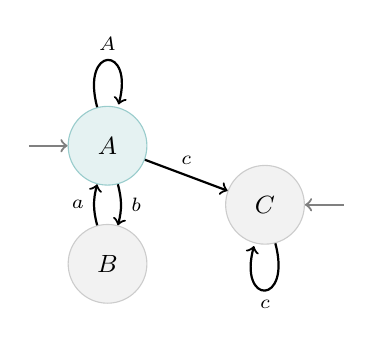
\begin{tikzpicture}[
    st/.style={draw, circle, minimum size=1cm, font=\small},
    arr/.style={->, thick}]
    
    \node[st, fill=teal!10, draw=teal!40] (q0) at (0,1.5) {$A$};
    \node[st, fill=gray!10, draw=gray!40] (q1) at (0,0) {$B$};
    \node[st, fill=gray!10, draw=gray!40] (q2) at (2,0.75) {$C$};
    
    \draw[->, gray, thick] (-1,1.5) -- (q0);
    \draw[->, gray, thick] (3,0.75) -- (q2);
    
    \draw[arr] (q0) edge [loop above] node {\scriptsize$A$} (q0);
    \draw[arr, bend left=15] (q0) to node [right] {\scriptsize$b$} (q1);
    \draw[arr, bend left=15] (q1) to node [left] {\scriptsize$a$} (q0);
    \draw[arr] (q0) -- node [above] {\scriptsize$c$} (q2);
    \draw[arr] (q2) edge [loop below] node {\scriptsize$c$} (q2);
\end{tikzpicture}
\end{minipage}\hfill
\begin{minipage}{0.55\textwidth}
\centering
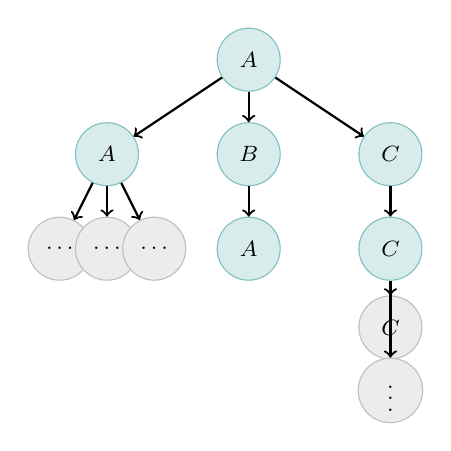
\begin{tikzpicture}[
    st/.style={draw, circle, minimum size=0.8cm, font=\footnotesize},
    arr/.style={->, thick}]
    
    \node[st, fill=teal!15, draw=teal!50] (r) at (0,0) {$A$};
    
    \node[st, fill=teal!15, draw=teal!50] (n0) at (-1.8,-1.2) {$A$};
    \node[st, fill=teal!15, draw=teal!50] (n1) at (0,-1.2) {$B$};
    \node[st, fill=teal!15, draw=teal!50] (n2) at (1.8,-1.2) {$C$};
    
    \node[st, fill=gray!15, draw=gray!50] (n00) at (-2.4,-2.4) {$\dots$};
    \node[st, fill=gray!15, draw=gray!50] (n01) at (-1.8,-2.4) {$\dots$};
    \node[st, fill=gray!15, draw=gray!50] (n02) at (-1.2,-2.4) {$\dots$};
    
    \node[st, fill=teal!15, draw=teal!50] (n10) at (0,-2.4) {$A$};
    
    \node[st, fill=teal!15, draw=teal!50] (n20) at (1.8,-2.4) {$C$};
    
    \node[st, fill=gray!15, draw=gray!50] (n200) at (1.8,-3.4) {$C$};
    \node[st, fill=gray!15, draw=gray!50] (n2000) at (1.8,-4.2) {$\vdots$};
    
    \draw[arr] (r) -- (n0);
    \draw[arr] (r) -- (n1);
    \draw[arr] (r) -- (n2);
    
    \draw[arr] (n0) -- (n00);
    \draw[arr] (n0) -- (n01);
    \draw[arr] (n0) -- (n02);
    
    \draw[arr] (n1) -- (n10);
    \draw[arr] (n2) -- (n20);
    \draw[arr] (n20) -- (n200);
    \draw[arr] (n20) -- (n2000);
\end{tikzpicture}
\end{minipage}
\caption{A transition system graph (left) and its infinite unfolding from initial state $A$ into a computation tree (right).}
\label{fig:unfolding}
\end{figure}

\aside{While an LTL formula evaluates a single path in isolation, a CTL formula can reason about the tree structure directly, using quantifiers like "for all paths ($\forall$)" or "there exists a path ($\exists$)" at each branching point.}

\subsection{Formalizing Trees: Domains and Valuations}
To study trees mathematically, we must formalize their structure. In words, positions are represented by the natural numbers $\{0, 1, 2, \dots\}$. In trees, a position (or node) is represented by a sequence of choices. For example, if we are in a binary tree, we can go left (0) or right (1). The sequence $010$ represents the node reached by going left, then right, then left.

This motivates the formal definition of a tree domain as a prefix-closed set of sequences.

\begin{definition}[$K$-ary Labeled Tree]
Let $A$ be a finite alphabet and let $K \ge 1$ be a natural number representing the maximum arity (branching factor) of the tree. A \emph{$K$-ary $A$-valued tree} $t$ is a labeling function:
$$t: \text{dom}(t) \to A$$
where the set of nodes $\text{dom}(t) \subseteq \{0, \dots, K-1\}^*$ is called the \emph{domain} of $t$. The domain must satisfy the following conditions:
\begin{enumerate}
    \item \textbf{Non-emptiness}: $\text{dom}(t) \neq \emptyset$, which implies that the root node $\epsilon$ (the empty word) always belongs to the domain.
    \item \textbf{Prefix Closure}: For every word $w \in \{0, \dots, K-1\}^*$ and symbol $j < K$, if $w j \in \text{dom}(t)$, then $w \in \text{dom}(t)$.
    \item \textbf{Width Closure (Child Ordering)}: For every word $w \in \{0, \dots, K-1\}^*$ and symbols $i, j < K$, if $w j \in \text{dom}(t)$ and $i < j$, then $w i \in \text{dom}(t)$.
\end{enumerate}
\end{definition}

\paragraph{Whiteboard Explanation of the Domain Conditions.}
Let us trace what these conditions mean operationally:
\begin{itemize}
    \item \textbf{Prefix closure} ensures that we cannot have "floating" nodes. If a node exists in the tree, its parent must also exist. You cannot reach a position like $01$ without first traversing through the root $\epsilon$ and the node $0$.
    \item \textbf{Width closure} ensures that children are ordered and contiguous starting from index $0$. An node cannot have a "second child" (labeled $j$) without also having all preceding children (labeled $i < j$). For instance, in a binary tree, we cannot have a right child ($w1$) unless the left child ($w0$) also exists.
\end{itemize}

\subsection{Paths, Subtrees, and Frontiers}
Now we define the key structural properties of a tree.

\begin{definition}[Paths and Subtrees]
Let $t$ be a $K$-ary $A$-valued tree:
\begin{itemize}
    \item A \emph{path} $\pi$ through $t$ is a maximal subset of $\text{dom}(t)$ that is linearly ordered by the prefix relation.
    \item For any node $w \in \text{dom}(t)$, the \emph{subtree} of $t$ at node $w$, denoted by $t|_w$, is the tree whose domain is:
    $$\text{dom}(t|_w) = \{ v \in \{0, \dots, K-1\}^* \mid w v \in \text{dom}(t) \}$$
    and whose labeling function is defined as $t|_w(v) = t(w v)$ for all $v \in \text{dom}(t|_w)$.
\end{itemize}
\end{definition}

\aside{Observe that the domain of a subtree $t|_w$ always resets to start at the empty word $\epsilon$. The root of the subtree is labeled with the value that $t$ had at position $w$.}

To define tree automata, we need to specify where the run of the automaton terminates or accepts. For a word of length $n$, the run is of length $n+1$, terminating at the position after the last letter. For trees, we generalize this using the concepts of \textbf{frontier} (the set of leaves) and \textbf{outer frontier} (the set of positions immediately below the leaves).

\begin{definition}[Frontiers]
Let $t$ be a $K$-ary $A$-valued tree:
\begin{itemize}
    \item The \emph{frontier} of $t$ (the set of leaves), denoted by $\text{fr}(t)$, is the set:
    $$\text{fr}(t) = \{ w \in \text{dom}(t) \mid \forall j < K, \, w j \notin \text{dom}(t) \}$$
    \item The \emph{outer frontier} of $t$, denoted by $\text{fr}^+(t)$, contains the positions immediately succeeding the leaves that are not part of the domain:
    $$\text{fr}^+(t) = \{ w j \in \{0, \dots, K-1\}^* \setminus \text{dom}(t) \mid w \in \text{dom}(t) \land j < K \}$$
    \item The \emph{extended domain} of $t$ is defined as $\text{dom}^+(t) = \text{dom}(t) \cup \text{fr}^+(t)$.
\end{itemize}
\end{definition}

To visualize these definitions, let us look at the finite binary tree ($K=2$) in Figure~\ref{fig:frontiers}.

\begin{figure}[H]
\centering
\begin{tikzpicture}[
    st/.style={draw, circle, minimum size=0.8cm, font=\footnotesize},
    leaf/.style={draw, circle, minimum size=0.8cm, font=\footnotesize, fill=teal!20, draw=teal!60, thick},
    outer/.style={draw, rectangle, minimum size=0.8cm, font=\footnotesize, fill=tomato!15, draw=tomato!50, dashed, thick},
    arr/.style={->, thick}]
    
    \node[st] (r) at (0,0) {$\epsilon$};
    \node[st] (n0) at (-1.5,-1) {$0$};
    \node[leaf] (n1) at (1.5,-1) {$1$};
    
    \node[leaf] (n00) at (-2.5,-2) {$00$};
    \node[leaf] (n01) at (-0.5,-2) {$01$};
    
    \node[outer] (o10) at (0.8,-2) {$10$};
    \node[outer] (o11) at (2.2,-2) {$11$};
    
    \node[outer] (o000) at (-3.2,-3) {$000$};
    \node[outer] (o001) at (-1.8,-3) {$001$};
    
    \node[outer] (o010) at (-1.2,-3) {$010$};
    \node[outer] (o011) at (0.2,-3) {$011$};
    
    \draw[arr] (r) -- (n0);
    \draw[arr] (r) -- (n1);
    \draw[arr] (n0) -- (n00);
    \draw[arr] (n0) -- (n01);
    
    \draw[arr, dashed, gray] (n1) -- (o10);
    \draw[arr, dashed, gray] (n1) -- (o11);
    \draw[arr, dashed, gray] (n00) -- (o000);
    \draw[arr, dashed, gray] (n00) -- (o001);
    \draw[arr, dashed, gray] (n01) -- (o010);
    \draw[arr, dashed, gray] (n01) -- (o011);
\end{tikzpicture}
\caption{A finite binary tree. The domain consists of $\{\epsilon, 0, 1, 00, 01\}$. The frontier (leaves) consists of $\{1, 00, 01\}$ (highlighted in teal). The outer frontier consists of $\{10, 11, 000, 001, 010, 011\}$ (dashed squares, highlighted in orange).}
\label{fig:frontiers}
\end{figure}

\subsection{Simplifying Focus: Binary Coding of K-ary Trees}
Studying $K$-ary trees for arbitrary $K$ complicates notations and proofs without adding conceptual value. Without loss of generality, we can restrict our study to \textbf{binary trees} ($K=2$). Any $K$-ary tree can be encoded into a binary tree over an extended alphabet by introducing a dummy padding symbol $\Omega$.

\begin{definition}[Binary Coding of $K$-ary Trees]
Let $t$ be a $K$-ary $A$-valued tree. Let $\Omega$ be a fresh symbol not in $A$. The binary coding of $t$ is a binary tree $t_{bin}: \text{dom}(t_{bin}) \to A \cup \{\Omega\}$ constructed as follows:
\begin{enumerate}
    \item We map each node $w = n_1 n_2 \dots n_r \in \text{dom}(t)$ (where $n_i < K$) to a binary sequence using the injection $f: \{0, \dots, K-1\}^* \to \{0,1\}^*$:
    $$f(n_1 n_2 \dots n_r) = 1^{n_1} 0 1^{n_2} 0 \dots 1^{n_r} 0$$
    where $1^k$ denotes $k$ consecutive $1$s.
    \item The domain $\text{dom}(t_{bin})$ is the prefix closure of the image $f(\text{dom}(t))$.
    \item The valuation $t_{bin}$ is defined as:
    $$t_{bin}(w') = \begin{cases} 
    t(w) & \text{if } w' = f(w) \text{ for some } w \in \text{dom}(t) \\ 
    \Omega & \text{otherwise} 
    \end{cases}$$
\end{enumerate}
\end{definition}

\begin{example}[Encoding a Node]
Let $K=3$ and consider a node $w = 2 0 1$ in the 3-ary tree. Its binary encoding is:
$$f(2 0 1) = 1^2 0 1^0 0 1^1 0 = 110010$$
At this position in the binary tree, $t_{bin}(110010) = t(201)$. The intermediate nodes along the path (such as $1$, $11$, $110$, $1100$, $11001$) are labeled with the dummy symbol $\Omega$.
\end{example}

\aside{This encoding is a prefix-preserving bijection between the original nodes and a subset of the binary tree. It can be extended to trees with countably infinite branching arity. Thus, we will assume all trees are binary ($K=2$) unless specified otherwise.}

From now on, we define:
\begin{itemize}
    \item $T(A)$ as the set of all finite binary $A$-valued trees.
    \item $T_\omega(A)$ as the set of all infinite binary $A$-valued trees (whose domain is $\{0,1\}^*$).
    \item $T_\infty(A) = T(A) \cup T_\omega(A)$ as the set of all binary $A$-valued trees.
\end{itemize}
A subset of $T(A)$ or $T_\omega(A)$ is called a \textbf{tree language}.

---

% =======================================================================
\section{Regular Tree Languages and Concatenation}
\label{sec:regular-tree-languages}

In the classical theory of formal languages over finite words, the Kleene theorem establishes a fundamental bridge between operational models (finite automata) and algebraic expressions (regular expressions). Regular expressions are built using three core operators: union, concatenation, and the Kleene star.

To generalize this framework to trees, we must redefine these algebraic operators. Union is straightforward: it is simply the set-theoretic union of tree languages. However, defining concatenation is not trivial. In words, a word has a single, unique end position where we can append another word. In contrast, a finite tree can have many leaves (its frontier). When we concatenate a tree $t'$ to a tree $t$, we must decide \emph{which} leaf of $t$ to replace.

To solve this, we define tree concatenation as a \textbf{substitution} operation. We designate specific symbols from a set of placeholders $C$ to represent "attachment points" on the leaves of the tree.

\subsection{Tree Concatenation (Substitution)}
Let $A$ be an alphabet and let $C$ be a set of placeholders disjoint from $A$. Trees are built over the alphabet $A \cup C$. Concatenation is defined with respect to a specific placeholder symbol $c \in C$.

\begin{definition}[Tree Concatenation]
Let $T \subseteq T(A \cup C)$ be a language of finite trees, and let $T' \subseteq T_\infty(A \cup C)$. The \emph{concatenation of $T'$ with $T$ with respect to $c$}, denoted by $T \cdot_c T'$, is the set of all trees obtained by taking a tree $t \in T$ and, for every leaf $w \in \text{fr}(t)$ labeled with $c$, substituting the leaf $w$ with a tree $t'_w \in T'$.

% Merged mathematical domain representation:
Mathematically, for each leaf $w$ labeled $c$, we can choose a different tree $t'_w \in T'$. The resulting tree $t_{new}$ has the domain:
$$\text{dom}(t_{new}) = \left( \text{dom}(t) \setminus \{ w \in \text{fr}(t) \mid t(w) = c \} \right) \cup \bigcup_{w \in \text{fr}(t), \, t(w) = c} \{ w v \mid v \in \text{dom}(t'_w) \}$$
and the valuation:
$$t_{new}(z) = \begin{cases}
t(z) & \text{if } z \in \text{dom}(t) \text{ and } z \text{ is not a descendant of any leaf labeled } c \\
t'_w(v) & \text{if } z = w v \text{ where } t(w) = c \text{ and } v \in \text{dom}(t'_w)
\end{cases}$$
\end{definition}

\begin{example}[Concatenation of Tree Languages]
Let $A = \{a, b, f\}$ and $C = \{c\}$. Let $T$ and $T'$ be two tree languages defined as:
$$T = \{ t_1, t_2 \}, \quad T' = \{ t_3, t_4 \}$$
where:
\begin{itemize}
    \item $t_1 = f(a, c)$ (a root $f$ with left child $a$ and right child $c$),
    \item $t_2 = b$ (a single leaf node labeled $b$),
    \item $t_3 = a$ (a single leaf node labeled $a$),
    \item $t_4 = f(b, b)$ (a root $f$ with two children labeled $b$).
\end{itemize}
Let us compute the concatenation $T \cdot_c T'$. For each tree in $T$:
\begin{itemize}
    \item For $t_2 = b$, there are no occurrences of the placeholder $c$ on the frontier. Thus, substitution yields the tree itself: $t_2 \cdot_c T' = \{b\}$.
    \item For $t_1 = f(a, c)$, the right child is labeled with the placeholder $c$. We substitute this leaf with any tree from $T'$. Since $T'$ contains two candidate trees, we obtain two possible trees:
    \begin{align*}
        t_{1a} &= f(a, t_3) = f(a, a) \\
        t_{1b} &= f(a, t_4) = f(a, f(b, b))
    \end{align*}
\end{itemize}
Taking the union of all possible resulting trees, we get:
$$T \cdot_c T' = \{ b, \, f(a, a), \, f(a, f(b, b)) \}$$
This example demonstrates that when concatenating sets of trees, different occurrences of the placeholder can be substituted by different elements from the target set, and trees without placeholders are preserved unchanged.
\end{example}

An intuitive visualization of this substitution is shown in Figure~\ref{fig:tree-concatenation}.

\begin{figure}[H]
\centering
\begin{tikzpicture}[
    st/.style={draw, circle, minimum size=0.8cm, font=\small},
    arr/.style={->, thick}]
    
    % Tree t
    \node[st] (t_r) at (0,0) {$f$};
    \node[st] (t_l) at (-0.8,-1) {$a$};
    \node[st, fill=tomato!20, draw=tomato!60, thick] (t_c) at (0.8,-1) {$c$};
    \draw[arr] (t_r) -- (t_l);
    \draw[arr] (t_r) -- (t_c);
    \node at (0,-1.7) {$t$};
    
    % Operator
    \node at (1.8,-0.5) {$\cdot_c$};
    
    % Tree t'
    \node[st] (tp_r) at (3,0) {$g$};
    \node[st] (tp_l) at (2.2,-1) {$b$};
    \node[st] (tp_r2) at (3.8,-1) {$b$};
    \draw[arr] (tp_r) -- (tp_l);
    \draw[arr] (tp_r) -- (tp_r2);
    \node at (3,-1.7) {$t'$};
    
    % Equals
    \node at (4.8,-0.5) {$=$};
    
    % Resulting tree
    \node[st] (tr_r) at (6.5,0) {$f$};
    \node[st] (tr_l) at (5.7,-1) {$a$};
    \node[st] (tr_c) at (7.3,-1) {$g$};
    \node[st] (tr_cl) at (6.5,-2) {$b$};
    \node[st] (tr_cr) at (8.1,-2) {$b$};
    \draw[arr] (tr_r) -- (tr_l);
    \draw[arr] (tr_r) -- (tr_c);
    \draw[arr] (tr_c) -- (tr_cl);
    \draw[arr] (tr_c) -- (tr_cr);
    \node at (6.9,-2.7) {$t \cdot_c t'$};
\end{tikzpicture}
\caption{Tree concatenation as substitution: the leaf labeled with the placeholder $c$ in tree $t$ is replaced by the tree $t'$.}
\label{fig:tree-concatenation}
\end{figure}

\subsection{Tree Kleene Star (Iterated Substitution)}
Having defined single substitution, we can now define iterated substitution. This corresponds to the Kleene star.

\begin{definition}[Tree Kleene Star]
Let $T \subseteq T(A \cup C)$ be a language of finite trees and let $c \in C$. The \emph{Kleene star of $T$ with respect to $c$}, denoted by $T^{*, c}$, is defined as the union:
$$T^{*, c} = \bigcup_{n \ge 0} T^{n, c}$$
where the sequence of approximations $T^{n, c}$ is defined inductively as:
\begin{align*}
    T^{0, c} &= \{c\} \\
    T^{n+1, c} &= T \cdot_c T^{n, c} \cup T^{n, c}
\end{align*}
\end{definition}

\begin{example}[Traces of the Tree Kleene Star]
Let $A = \{a, f\}$ and $C = \{c\}$, and let $T = \{ f(c, c), a \}$. Let us trace the approximations $T^{n, c}$ for the iterated substitution $T^{*, c}$:
\begin{itemize}
    \item \textbf{Base Case ($n=0$)}:
    $$T^{0, c} = \{c\}$$
    This represents a single root node labeled with the placeholder $c$.
    
    \item \textbf{First Iteration ($n=1$)}:
    $$T^{1, c} = T \cdot_c T^{0, c} \cup T^{0, c} = \{ f(c, c), a \} \cdot_c \{c\} \cup \{c\} = \{ f(c, c), a, c \}$$
    
    \item \textbf{Second Iteration ($n=2$)}:
    $$T^{2, c} = T \cdot_c T^{1, c} \cup T^{1, c}$$
    To compute $T \cdot_c T^{1, c}$, we take each tree in $T$ and replace its $c$-leaves with any choice from $T^{1, c} = \{ f(c, c), a, c \}$:
    \begin{itemize}
        \item For $a \in T$, there are no $c$ leaves, so we get $\{a\}$.
        \item For $f(c, c) \in T$, we have two leaves labeled $c$. We can replace them independently with any combination of trees from $\{ f(c, c), a, c \}$. This yields:
        \begin{itemize}
            \item Replacing both with $a$: $f(a, a)$
            \item Replacing left with $a$, right with $c$: $f(a, c)$
            \item Replacing left with $c$, right with $a$: $f(c, a)$
            \item Replacing left with $a$, right with $f(c, c)$: $f(a, f(c, c))$
            \item Replacing both with $f(c, c)$: $f(f(c, c), f(c, c))$
            \item \dots and so on, for all 9 possible combinations.
        \end{itemize}
    \end{itemize}
    Taking the union with $T^{1, c}$, we see that $T^{2, c}$ contains trees of varying shapes and branching configurations (such as $f(a, c)$ where one branch stopped growing while the other was replaced by the placeholder $c$, or $f(a, a)$ where all placeholders have been resolved to terminals).
\end{itemize}
\end{example}

\begin{formaldetails}[Why is the Tree Kleene Star Cumulative?]
Observe that in the inductive step, we define $T^{n+1, c}$ by taking the union with $T^{n, c}$ (making the sequence cumulative). This is in stark contrast to words, where the Kleene star is defined by simply concatenating $n+1$ words, and the union is taken only at the very end.

Why is this cumulative union required for trees?
In words, concatenation only occurs at the single end of the string, meaning all parts of the word grow uniformly in length. In trees, however, each step of the substitution replaces \emph{all} occurrences of the placeholder $c$ on the frontier.
If we did not include the cumulative union $T^{n, c}$ at each step, we would be forced to substitute $c$ at all leaves at the exact same iteration step. This would imply that all branches of the tree must grow to the exact same depth, preventing us from generating trees with branches of different lengths (e.g., one branch terminating early while another continues to branch). Including $T^{n, c}$ in the inductive step acts as a "stopping option" for any leaf labeled $c$, allowing different branches to decouple their growth and generate arbitrary irregular tree shapes.
\end{formaldetails}

\subsection{Regular Tree Languages}
With these definitions, we can now formalize regular tree languages over finite trees.

\begin{definition}[Regular Tree Language]
A tree language $T \subseteq T(A)$ is \emph{regular} if and only if there exists a finite set of placeholder symbols $C$ disjoint from $A$ such that $T$ can be obtained from finite subsets of $T(A \cup C)$ by applying a finite number of times the operations of:
\begin{enumerate}
    \item Union ($T_1 \cup T_2$),
    \item Concatenation with respect to $c \in C$ ($T_1 \cdot_c T_2$),
    \item Kleene star with respect to $c \in C$ ($T_1^{*, c}$).
\end{enumerate}
\end{definition}

\begin{example}[Algebraic Expression for All Finite Binary Trees]
Suppose we want to define the language of all finite binary trees over the alphabet $A = \{a, b\}$. A tree in this language is either a single terminal leaf (labeled $a$ or $b$) or a node (labeled $a$ or $b$) with two child subtrees which are themselves finite binary trees.

Using a single placeholder $c$, we can define the finite set of base trees:
$$B = \{ a, \, b, \, a(c, c), \, b(c, c) \}$$
The regular tree language $B^{*, c}$ contains exactly all finite binary trees over $A$. Let's see why:
\begin{itemize}
    \item At each step of the Kleene star substitution, we can choose to replace the active placeholder leaves $c$ either with terminals $a$ or $b$ (which terminates that branch), or with branching patterns $a(c, c)$ or $b(c, c)$ (which extends the branch and introduces new placeholders).
    \item For example, the tree $a(b, a(b, b))$ is generated by:
    $$c \xrightarrow{B} a(c, c) \xrightarrow{B} a(b, c) \xrightarrow{B} a(b, a(c, c)) \xrightarrow{B} a(b, a(b, b))$$
    which belongs to $B^{4, c} \subseteq B^{*, c}$.
    \item Since all placeholders are eventually replaced by $a$ or $b$, the final trees contain only symbols from $A$, making $B^{*, c}$ a valid regular tree language over $A$.
\end{itemize}
\end{example}

\aside{Since the final regular language $T$ is a subset of $T(A)$, it consists only of trees labeled by $A$. This implies that all placeholder symbols from $C$ must be completely substituted away during the algebraic construction.}

\subsection{Tuple Concatenation and Omega-Closure}
In many constructions, we need to perform simultaneous substitution of multiple different placeholder symbols. This is modeled by \textbf{tuple concatenation}.

\begin{definition}[Tuple Concatenation]
Let $C = \{c_1, \dots, c_m\}$ be a set of placeholders. Let $T \subseteq T(A \cup C)$ and let $T_1, \dots, T_m \subseteq T_\infty(A \cup C)$ be tree languages. The \emph{tuple concatenation}, denoted by:
$$T \cdot_{\bar{c}} (T_1, \dots, T_m)$$
is the tree language obtained by taking a tree $t \in T$ and, for each $i \in \{1, \dots, m\}$, replacing every leaf labeled $c_i$ on the frontier of $t$ with some tree from $T_i$.
\end{definition}

Using tuple concatenation, we can define the infinite iteration of tree substitution, leading to the \textbf{$\omega$-closure} of tree languages, which is the algebraic representation of infinite trees.

\begin{definition}[Tree Omega-Closure]
Let $C = \{c_1, \dots, c_m\}$ be placeholders. Let $T_1, \dots, T_m \subseteq T(A \cup C)$ be languages of finite trees. The \emph{$\omega$-closure} with respect to $\bar{c}$, denoted by:
$$(T_1, \dots, T_m)^{\omega, \bar{c}}$$
is the set of all infinite trees obtained by applying the tuple concatenation infinitely many times starting from the initial set of placeholders.
\end{definition}

\begin{example}[Alternating Paths via Omega-Closure]
Suppose we want to generate the set of all infinite binary trees where every path alternates between the symbols $a$ and $b$, starting with $a$ at the root. We can define this language algebraically.
Let $C = \{c_a, c_b\}$ be placeholders. We define the base sets:
\begin{align*}
    T_a &= \{ a(c_b, c_b) \} \\
    T_b &= \{ b(c_a, c_a) \}
\end{align*}
The language of alternating trees is exactly the $\omega$-closure:
$$T_{alt} = (T_a, T_b)^{\omega, (c_a, c_b)}$$
In this construction, we start with the placeholder $c_a$. It is replaced by $a(c_b, c_b)$ (which introduces $c_b$ at both children). In the next step, both occurrences of $c_b$ are replaced by $b(c_a, c_a)$, which introduces $c_a$ at all four grandchildren. Repeating this infinitely yields an infinite binary tree where every path alternates $a$ and $b$.
\end{example}

\subsection{Concatenation of Infinite Trees}
If a tree is infinite, it does not have a frontier (its set of leaves is empty). How can we define concatenation for infinite trees?

To solve this, we define concatenation by substituting the \emph{first} occurrence of the placeholder $c$ along each path.
\begin{definition}[Infinite Tree Concatenation]
Let $t \in T_\omega(A \cup C)$ be an infinite tree, and let $T' \subseteq T_\omega(A \cup C)$. The concatenation $t \cdot_c T'$ is the set of trees obtained by replacing the subtree $t|_w$ with some tree in $T'$ for each minimal node $w \in \text{dom}(t)$ (with respect to prefix ordering) such that $t(w) = c$.
\end{definition}

This ensures that we perform substitution at the boundary where the placeholder $c$ first appears along each infinite history.

---

% =======================================================================
\section{Tree Automata on Finite Trees}
\label{sec:tree-automata-finite}

Having established the algebraic representation of tree languages (regular tree expressions), we now introduce the corresponding operational model: \textbf{tree automata}.

Just as a standard automaton processes a word by reading symbols sequentially and transitioning between states, a tree automaton processes a tree by traversing its branching structure. Over finite trees, we can process the structure in two directions:
\begin{enumerate}
    \item \textbf{Top-Down}: We start at the root and work down towards the leaves. At each node, the automaton reads the label and splits its state, spawning two independent state processes to run on the left and right child subtrees.
    \item \textbf{Bottom-Up}: We start at the leaves (outer frontier) and work up towards the root. At each node, the automaton reads the states reached by its children and combines them with the current node's label to produce a state for the parent.
\end{enumerate}

As we will see, this choice of direction represents a crucial fork in the road: top-down deterministic automata are strictly weaker than their non-deterministic counterparts, whereas bottom-up deterministic and non-deterministic automata are expressively equivalent.

\subsection{Top-Down Tree Automata}
We begin by defining the top-down model.

\begin{definition}[Non-deterministic Top-down Tree Automaton]
A \emph{non-deterministic top-down tree automaton} (NTTA) over finite binary trees is a tuple:
$$A = (Q, \Sigma, Q_0, \Delta, F)$$
where:
\begin{itemize}
    \item $Q$ is a finite set of states,
    \item $\Sigma$ is the input alphabet,
    \item $Q_0 \subseteq Q$ is the set of initial states (applied at the root),
    \item $F \subseteq Q$ is the set of final states (checked at the leaves),
    \item $\Delta \subseteq Q \times \Sigma \times Q \times Q$ is the transition relation.
\end{itemize}
A transition $(q, a, q_L, q_R) \in \Delta$ (often written $q \xrightarrow{a} (q_L, q_R)$) means that if the automaton is in state $q$ at a node labeled $a$, it sends state $q_L$ to the left child and state $q_R$ to the right child.
\end{definition}

\begin{definition}[NTTA Run and Acceptance]
Let $t \in T(\Sigma)$ be a finite binary tree. A \emph{run} of the NTTA $A$ on $t$ is a tree $R: \text{dom}^+(t) \to Q$ labeled with states, which is defined over the extended domain of $t$, satisfying:
\begin{enumerate}
    \item \textbf{Initiality}: The root of the run is labeled with an initial state:
    $$R(\epsilon) \in Q_0$$
    \item \textbf{Consequentiality}: For every node $w \in \text{dom}(t)$ (excluding the outer frontier), the transitions must obey the transition relation:
    $$(R(w), t(w), R(w0), R(w1)) \in \Delta$$
\end{enumerate}
The run $R$ is \emph{successful} if all leaves of the run (which are the nodes in the outer frontier of $t$) are labeled with final states:
$$\forall w \in \text{fr}^+(t), \, R(w) \in F$$
The tree $t$ is accepted by $A$ if there exists at least one successful run of $A$ on $t$. The language recognized by $A$ is denoted by $L(A)$.
\end{definition}

\aside{Notice that the run $R$ is defined on the extended domain $\text{dom}^+(t) = \text{dom}(t) \cup \text{fr}^+(t)$. This is because, like in the case of finite words, we need an extra "look-ahead" step at the leaves to check if we can transition into final states.}

\begin{example}[NTTA Run Visualization]
Let us visualize a run on the tree $t = f(a, b)$, which has the domain $\text{dom}(t) = \{\epsilon, 0, 1\}$ and outer frontier $\text{fr}^+(t) = \{00, 01, 10, 11\}$. 

A run $R$ of the automaton must assign states to all nodes in $\text{dom}^+(t)$, as shown in Figure~\ref{fig:run-tree-comparison}.

\begin{figure}[H]
\centering
\begin{minipage}{0.45\textwidth}
\centering
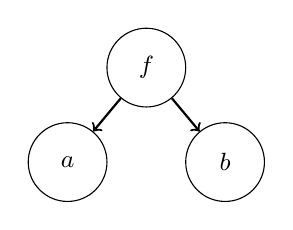
\begin{tikzpicture}[
    st/.style={draw, circle, minimum size=1cm, font=\small},
    arr/.style={->, thick}]
    
    \node[st] (r) at (0,0) {$f$};
    \node[st] (l) at (-1,-1.2) {$a$};
    \node[st] (rt) at (1,-1.2) {$b$};
    
    \draw[arr] (r) -- (l);
    \draw[arr] (r) -- (rt);
\end{tikzpicture}
\caption*{Input Tree $t$}
\end{minipage}\hfill
\begin{minipage}{0.45\textwidth}
\centering
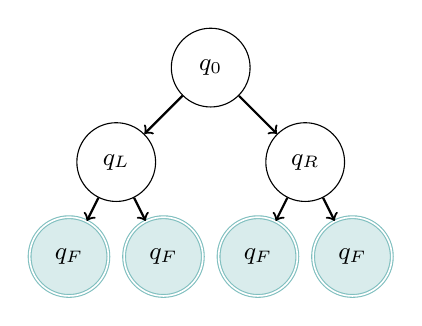
\begin{tikzpicture}[
    st/.style={draw, circle, minimum size=1cm, font=\small},
    acc/.style={draw, circle, minimum size=1cm, font=\small, double, fill=teal!15, draw=teal!50},
    arr/.style={->, thick}]
    
    \node[st] (r) at (0,0) {$q_0$};
    \node[st] (l) at (-1.2,-1.2) {$q_L$};
    \node[st] (rt) at (1.2,-1.2) {$q_R$};
    
    \node[acc] (ll) at (-1.8,-2.4) {$q_F$};
    \node[acc] (lr) at (-0.6,-2.4) {$q_F$};
    \node[acc] (rl) at (0.6,-2.4) {$q_F$};
    \node[acc] (rr) at (1.8,-2.4) {$q_F$};
    
    \draw[arr] (r) -- (l);
    \draw[arr] (r) -- (rt);
    \draw[arr] (l) -- (ll);
    \draw[arr] (l) -- (lr);
    \draw[arr] (rt) -- (rl);
    \draw[arr] (rt) -- (rr);
\end{tikzpicture}
\caption*{Run Tree $R$}
\end{minipage}
\caption{Side-by-side comparison of an input tree $t$ of height 1 and its corresponding run tree $R$ of height 2 over the extended domain.}
\label{fig:run-tree-comparison}
\end{figure}
\end{example}

\subsection{The Expressive Limit of Deterministic Top-Down Automata}
A top-down tree automaton is \textbf{deterministic} (DTTA) if:
\begin{enumerate}
    \item There is exactly one initial state: $|Q_0| = 1$,
    \item For every state $q \in Q$ and symbol $a \in \Sigma$, there is \emph{at most one} pair $(q_L, q_R) \in Q \times Q$ such that $(q, a, q_L, q_R) \in \Delta$.
\end{enumerate}

In the case of finite words, deterministic and non-deterministic finite automata (DFAs and NFAs) are equivalent. Surprisingly, this equivalence breaks for top-down tree automata. We first demonstrate a language that is easily recognizable deterministically, and then a language that highlights the limit of top-down determinism.

\begin{example}[Path Property: Deterministic Top-Down Tree Automaton]
Let $\Sigma = \{a, b\}$ and consider the language $T_{\ge 1, a}$ of all finite binary trees where \emph{every} path from the root to a leaf contains at least one node labeled $a$.
We can design a DTTA for $T_{\ge 1, a}$ as follows:
\begin{itemize}
    \item States: $Q = \{q_0, q_a\}$, where $q_0$ represents the state before seeing an $a$ on the path, and $q_a$ represents the state after seeing an $a$.
    \item Initial state: $Q_0 = \{q_0\}$.
    \item Final states: $F = \{q_a\}$ (meaning we must have seen an $a$ before reaching the leaf).
    \item Transitions:
    \begin{align*}
        q_0 \xrightarrow{a} (q_a, q_a) & \quad \text{and} \quad q_0 \xrightarrow{b} (q_0, q_0) \\
        q_a \xrightarrow{a} (q_a, q_a) & \quad \text{and} \quad q_a \xrightarrow{b} (q_a, q_a)
    \end{align*}
\end{itemize}
Let us trace this automaton on a tree. At the root, we start in $q_0$. If we see $b$, we propagate $q_0$ down to both children. If we see $a$, we transition to $q_a$ and propagate $q_a$ down. Once a branch transitions to $q_a$, it stays in $q_a$ regardless of subsequent labels. Since we check that all leaves in the outer frontier are in $F = \{q_a\}$, the tree is accepted if and only if every single path contains at least one $a$. This automaton is deterministic because for each state and label, there is exactly one target pair.
\end{example}

\begin{theorem}[Top-Down Deterministic Limit]
Deterministic top-down tree automata (DTTA) are strictly less expressive than non-deterministic top-down tree automata (NTTA):
$$\text{DTTA} \subset \text{NTTA}$$
\end{theorem}

\begin{proof}
Clearly, \text{DTTA} $\subseteq$ \text{NTTA} by definition. To prove that the inclusion is strict, we show that the finite tree language:
$$T_{xor} = \{ f(a, b), \, f(b, a) \}$$
is recognizable by an NTTA but cannot be recognized by any DTTA.
\begin{enumerate}
    \item \textbf{NTTA Construction}: We construct an NTTA with states $Q = \{q_0, q_a, q_b, q_F\}$, initial state $Q_0 = \{q_0\}$, final states $F = \{q_F\}$, and transitions:
    \begin{align*}
        q_0 &\xrightarrow{f} (q_a, q_b) \quad \text{and} \quad q_0 \xrightarrow{f} (q_b, q_a) \\
        q_a &\xrightarrow{a} (q_F, q_F) \\
        q_b &\xrightarrow{b} (q_F, q_F)
    \end{align*}
    This automaton easily accepts $f(a,b)$ by choosing the first transition, and $f(b,a)$ by choosing the second transition. All other runs get stuck and reject. Thus, $L(A) = T_{xor}$.
    
    \item \textbf{Proof of Unrecognizability by DTTA}: Assume for contradiction that there exists a DTTA $A' = (Q', \Sigma, \{q'_0\}, \delta', F')$ recognizing $T_{xor}$.
    Since $f(a,b) \in L(A')$, there must exist a unique transition for the root:
    $$q'_0 \xrightarrow{f} (q'_L, q'_R)$$
    such that $q'_L$ accepts the left child leaf $a$ and $q'_R$ accepts the right child leaf $b$. This means:
    $$(q'_L, a, q'_F, q'_F) \in \delta' \quad \text{and} \quad (q'_R, b, q'_F, q'_F) \in \delta'$$
    for some final states in $F'$.
    
    Similarly, since $f(b,a) \in L(A')$, the same unique root transition $q'_0 \xrightarrow{f} (q'_L, q'_R)$ must be used (as $A'$ is deterministic). This implies that $q'_L$ must accept the leaf $b$ and $q'_R$ must accept the leaf $a$:
    $$(q'_L, b, q'_F, q'_F) \in \delta' \quad \text{and} \quad (q'_R, a, q'_F, q'_F) \in \delta'$$
    
    Now, consider the trees $t_{aa} = f(a, a)$ and $t_{bb} = f(b, b)$.
    If we run $A'$ on $t_{aa}$, the root transitions to $(q'_L, q'_R)$. The state $q'_L$ accepts the left leaf $a$ (since $q'_L$ accepts $a$), and the state $q'_R$ accepts the right leaf $a$ (since $q'_R$ accepts $a$). Thus, $A'$ accepts $t_{aa}$.
    By symmetric reasoning, $A'$ also accepts $t_{bb}$.
    However, $t_{aa}, t_{bb} \notin T_{xor}$. This is a contradiction, since $L(A') = T_{xor}$.
\end{enumerate}
Thus, no DTTA can recognize $T_{xor}$, proving $\text{DTTA} \subset \text{NTTA}$.
\end{proof}

\aside{Why does determinism fail top-down? 
A top-down automaton is forced to split its state at a node \emph{before} it reads the leaves below. A deterministic automaton cannot relate the choices made on the left branch with the choices made on the right branch; once the split happens, the two branches run in complete isolation. Non-determinism bypasses this by allowing the automaton to guess the global correlation (e.g., guessing whether the tree is $f(a,b)$ or $f(b,a)$) at the root.}

\subsection{Bottom-Up Tree Automata}
To restore the equivalence between determinism and non-determinism, we turn to the \textbf{bottom-up} model. A bottom-up automaton reads the tree starting from the leaves and moves up to the root.

\begin{definition}[Non-deterministic Bottom-up Tree Automaton]
A \emph{non-deterministic bottom-up tree automaton} (NBTA) over finite binary trees is a tuple:
$$A = (Q, \Sigma, Q_0, \Delta, F)$$
where:
\begin{itemize}
    \item $Q$ is a finite set of states,
    \item $\Sigma$ is the input alphabet,
    \item $Q_0 \subseteq Q$ is the set of initial states (applied at the outer frontier),
    \item $F \subseteq Q$ is the set of final states (checked at the root),
    \item $\Delta \subseteq Q \times Q \times \Sigma \times Q$ is the transition relation.
\end{itemize}
A transition $(q_L, q_R, a, q) \in \Delta$ (written $(q_L, q_R) \xrightarrow{a} q$) means that if the left child is in state $q_L$, the right child is in state $q_R$, and the parent node is labeled $a$, the parent transitions to state $q$.
\end{definition}

\begin{definition}[NBTA Run and Acceptance]
Let $t \in T(\Sigma)$ be a finite binary tree. A \emph{run} of the NBTA $A$ on $t$ is a tree $R: \text{dom}^+(t) \to Q$ satisfying:
\begin{enumerate}
    \item \textbf{Initiality}: All leaf nodes of the run (the outer frontier $\text{fr}^+(t)$) are labeled with initial states:
    $$\forall w \in \text{fr}^+(t), \, R(w) \in Q_0$$
    \item \textbf{Consequentiality}: For every node $w \in \text{dom}(t)$, the parent state $R(w)$ is determined by the children's states $R(w0), R(w1)$ and the node label $t(w)$:
    $$(R(w0), R(w1), t(w), R(w)) \in \Delta$$
\end{enumerate}
The run $R$ is \emph{successful} if the root node of the run is labeled with a final state:
$$R(\epsilon) \in F$$
\end{definition}

A bottom-up tree automaton is \textbf{deterministic} (DBTA) if $|Q_0| = 1$ and for every $q_L, q_R \in Q$ and $a \in \Sigma$, there is \emph{at most one} state $q \in Q$ such that $(q_L, q_R, a, q) \in \Delta$.

\subsection{Bottom-Up Determinization (Subset Construction)}
Unlike the top-down case, bottom-up tree automata can always be determinized. This is because a bottom-up transition can collect and merge information from the children as it propagates upwards.

\begin{theorem}[Bottom-Up Determinization]
Deterministic bottom-up tree automata (DBTA) are expressively equivalent to non-deterministic bottom-up tree automata (NBTA):
$$\text{DBTA} \equiv \text{NBTA}$$
\end{theorem}

\begin{proof}
Clearly, $\text{DBTA} \subseteq \text{NBTA}$. To prove the converse, let $A = (Q, \Sigma, Q_0, \Delta, F)$ be an NBTA. We construct an equivalent DBTA $A' = (Q', \Sigma, Q'_0, \delta', F')$ using a generalization of the subset construction:
\begin{itemize}
    \item \textbf{States}: $Q' = \mathcal{P}(Q)$ (the power set of $Q$).
    \item \textbf{Initial State}: $Q'_0 = \{ Q_0 \}$ (the single initial state of $A'$ is the set of all initial states of $A$).
    \item \textbf{Transition Function}: For any subset of states $S_L, S_R \subseteq Q$ and symbol $a \in \Sigma$:
    $$\delta'(S_L, S_R, a) = \{ q \in Q \mid \exists q_L \in S_L, \, q_R \in S_R \text{ such that } (q_L, q_R, a, q) \in \Delta \}$$
    \item \textbf{Final States}: $F' = \{ S \subseteq Q \mid S \cap F \neq \emptyset \}$.
\end{itemize}
We prove by induction on the height of the tree $t$ that the state reached at the root of $t$ in the unique run of $A'$ is exactly the set of all states that can be reached at the root of $t$ in some run of $A$.
\begin{itemize}
    \item \textbf{Base Case}: Let $t$ be a single leaf labeled $a$ (height 0). The domain is $\{\epsilon\}$ and the outer frontier is $\{0, 1\}$. 
    In the DBTA $A'$, the children $0$ and $1$ are labeled with $Q_0$. The root transitions to:
    $$S' = \delta'(Q_0, Q_0, a) = \{ q \in Q \mid \exists q_L, q_R \in Q_0, \, (q_L, q_R, a, q) \in \Delta \}$$
    This is precisely the set of states that the NBTA $A$ can reach at the root of $t$ starting from initial states in the outer frontier.
    
    \item \textbf{Inductive Step}: Let $t = a(t_L, t_R)$ be a tree where the subtrees $t_L, t_R$ have height at most $h$.
    By the induction hypothesis, the unique run of $A'$ on $t_L$ (resp. $t_R$) reaches the subset of states $S_L$ (resp. $S_R$), which contains exactly the states reachable by $A$ at the root of $t_L$ (resp. $t_R$).
    When evaluating the root of $t$, the DBTA $A'$ computes:
    $$S' = \delta'(S_L, S_R, a)$$
    By definition of $\delta'$, $q \in S'$ if and only if there exist $q_L \in S_L$ and $q_R \in S_R$ such that $(q_L, q_R, a, q) \in \Delta$. Since $S_L$ and $S_R$ are the exact sets of reachable states for $t_L$ and $t_R$, $S'$ is the exact set of states that $A$ can reach at the root of $t$.
\end{itemize}
Finally, $A'$ accepts $t \iff S' \in F' \iff S' \cap F \neq \emptyset$, which is true if and only if there exists a successful run of $A$ on $t$. Thus, $L(A') = L(A)$.
\end{proof}

\begin{example}[Determinizing the NBTA for $T_{xor}$]
Let us trace the subset construction on the NBTA for $T_{xor} = \{ f(a,b), f(b,a) \}$.
Recall the NBTA states are $Q = \{q_0, q_a, q_b, q_{acc}\}$, with $Q_0 = \{q_F\}$, $F = \{q_{acc}\}$, and transitions:
\begin{align*}
    (q_F, q_F) &\xrightarrow{a} q_a \\
    (q_F, q_F) &\xrightarrow{b} q_b \\
    (q_a, q_b) &\xrightarrow{f} q_{acc} \\
    (q_b, q_a) &\xrightarrow{f} q_{acc}
\end{align*}
We construct the DBTA $A'$:
\begin{itemize}
    \item The initial state of $A'$ is the set $S_0 = \{q_F\}$.
    \item If we evaluate a leaf node labeled $a$, its children (in the outer frontier) are in state $S_0 = \{q_F\}$. The DBTA transitions to:
    $$\delta'( \{q_F\}, \{q_F\}, a ) = \{ q \in Q \mid (q_F, q_F) \xrightarrow{a} q \} = \{ q_a \}$$
    \item Similarly, for a leaf node labeled $b$, the DBTA transitions to:
    $$\delta'( \{q_F\}, \{q_F\}, b ) = \{ q \in Q \mid (q_F, q_F) \xrightarrow{b} q \} = \{ q_b \}$$
    \item Now, consider the root node labeled $f$ of the tree $t = f(a,b)$. The left subtree (leaf $a$) reaches state $\{q_a\}$, and the right subtree (leaf $b$) reaches state $\{q_b\}$. The DBTA transitions to:
    $$\delta'( \{q_a\}, \{q_b\}, f ) = \{ q \in Q \mid \exists q_L \in \{q_a\}, q_R \in \{q_b\} \text{ s.t. } (q_L, q_R) \xrightarrow{f} q \} = \{ q_{acc} \}$$
    \item For the tree $t' = f(b,a)$, the left subtree reaches state $\{q_b\}$, and the right subtree reaches state $\{q_a\}$. The DBTA transitions to:
    $$\delta'( \{q_b\}, \{q_a\}, f ) = \{ q_{acc} \}$$
    \item If we have $t_{aa} = f(a,a)$, both children reach state $\{q_a\}$. The transition evaluates to:
    $$\delta'( \{q_a\}, \{q_a\}, f ) = \emptyset$$
    which is not an accepting state because $\emptyset \cap \{q_{acc}\} = \emptyset$.
\end{itemize}
Since $\{q_{acc}\} \cap F \neq \emptyset$, the DBTA accepts $f(a,b)$ and $f(b,a)$ but rejects $f(a,a)$ and $f(b,b)$ as desired, successfully determinizing the system.
\end{example}

\subsection{Decision Problems and Closure Properties}
We conclude this section by stating the algorithmic and algebraic properties of finite tree languages.

\begin{theorem}[Decidability of Emptiness]
The emptiness problem for tree automata (top-down or bottom-up) is decidable in polynomial time.
\end{theorem}

\begin{proof}
We can solve the emptiness problem by computing the set of reachable states in a bottom-up fashion. Let $A = (Q, \Sigma, Q_0, \Delta, F)$ be an NBTA. We define the sequence of sets of reachable states $Reach_i \subseteq Q$:
\begin{align*}
    Reach_0 &= Q_0 \\
    Reach_{i+1} &= Reach_i \cup \{ q \in Q \mid \exists q_L, q_R \in Reach_i, \, a \in \Sigma \text{ such that } (q_L, q_R, a, q) \in \Delta \}
\end{align*}
Since $Q$ is finite, this sequence must reach a fixed point in at most $|Q|$ steps, i.e., $Reach_k = Reach_{k+1}$ for some $k \le |Q|$. The language $L(A)$ is non-empty if and only if:
$$Reach_k \cap F \neq \emptyset$$
This fixed-point computation can be performed in time polynomial in the size of the transition relation.
\end{proof}

\begin{summarybox}[Small Model Property]
The fixed-point reachability algorithm implies a \textbf{small model property} for finite trees: if a tree language recognized by a tree automaton is non-empty, then it contains a tree of height at most $|Q|$.
\end{summarybox}

Finally, we state the equivalence between the algebraic and operational models, which is the tree-counterpart to Kleene's theorem.

\begin{theorem}[Kleene's Theorem for Trees]
A tree language $T \subseteq T(A)$ is regular if and only if it is recognized by a finite tree automaton.
\end{theorem}

\begin{corollary}[Boolean Closure]
The class of regular tree languages is closed under all Boolean operations (union, intersection, and complementation) and projection.
\end{corollary}

\begin{proof}[Proof Sketch]
Union and intersection are achieved via standard product constructions. Complementation is achieved by first determinizing the bottom-up tree automaton (via the subset construction) and then complement at the root: $F^C = \mathcal{P}(Q) \setminus F'$.
\end{proof}

